\chapter{Implementation einer AR Anwendung für Android}
Im Rahmen des Praxisteils dieser Arbeit ist eine Applikation für Android basierte Smartphones erstellt worden. In diesem Praxisteil werden die verwendeten Tools und Frameworks, um die Augmented Reality Anwendung zu erstellen, beschrieben. Das im folgenden vorgestellte Framework ARCore, implementiert den Simultaneus Location and Mapping Ansatz und ist als einzige AR-Programmierschnittstelle Open Source (Siehe Tabelle S.29).



\section{ARCore}
ARCore, das von Google entwickelt wird und das seit März 2018 verfügbar ist, ist der Nachfolger des ebenfalls von Google ins Leben gerufene Projekt Tango, welches jedoch spezielle \glqq Time-of-flight\grqq{} (TOF) Kameras benötigt, um Distanzen im Raum mithilfe des Lichtlaufzeitverfahrens zu messen. Dieser Ansatz hat sich wegen der fehlenden technischen Voraussetzungen der meisten Android Geräte nicht durchgesetzt. Da Google mit dem von Apple veröffentlichen Framework ARKit schritt halten wollte, wurde Projekt Tango beendet und durch ARCore ersetzt. ARCore verwendet drei Schlüsselfunktionen um virtuelle Objekte in die reale Welt zu integrieren (vgl. \cite{arcore}):

\begin{itemize}
\item \textbf{Motion Tracking} ermöglicht es dem Smartphone seine Position relativ zur Umgebung zu verfolgen und zu verstehen.

\item \textbf{Environmental understanding} ermöglicht es dem Smartphone die Größe und Lage aller Arten von Oberflächen  zu erfassen, dazu zählen horizontale, vertikale oder schräge Oberflächen.

\item \textbf{Light estimation} ermöglicht die Abschätzung der aktuellen Lichtverhältnisse in der Umgebung, zur korrekten Beleuchtung und zur Erstellung von Schatten.
\end{itemize}

\subsection{Unterstütze Geräte}
Um eine gute und flüssige Erfahrung für den Endnutzer zu gewährleisten, müssen unterstützte Smartphones bestimmte Kriterien erfüllen. Dazu zählen die Qualität der verbauten Kamera, der Bewegungssensoren und der Designarchitektur. Weiterhin muss das Gerät über eine leistungsstarke CPU verfügen, die sich in das Hardware-Design integriert, um gute Leistung und effektive Echtzeitberechnung zu gewährleisten. Die Voraussetzungen um ARCore zu verwenden, werden wie folgt betitelt:

\begin{itemize}
\item \textbf{Android 7.0} oder höher. (Einige Modelle benötigen neuere Versionen)
\item Ein Gerät, das ursprünglich mit dem \textbf{Google Play Store} ausgeliefert wurde.
\item \textbf{Internetzugang}, um Google Play Services für AR zu installieren oder zu aktualisieren.
\end{itemize}

Aktuell werden 144 Android Smartphones, die mit dem Google Play Store ausgeliefert werden unterstützt. Weiterhin werden 29 chinesische Modelle unterstützt, bei welchen die Google Play Services manuell über die App Stores der Hersteller installiert werden müssen. Auch 20 iOS Smartphone Modelle werden unterstützt, dabei benötigt ARCore jedoch ARKit kompatible Geräte mit iOS 11.0 oder höher (Stand 22.08.2019, vgl. \cite{arcore_devices}).

\subsection{Grundlegende Konzepte}

In diesem Abschnitt werden grundlegende Funktionen, die ARCore bietet, erläutert.

\textbf{Motion Tracking} wird in ARCore mit einem Prozess namens \glqq Concurrent Odometry and Mapping\grqq{} (COM) ermöglicht. Dabei werden Features im Kamerabild erkannt und zur Bestimmung der Änderung der Position des Smartphones verwendet. Diese visuellen Informationen werden mit Trägheitsmessungen der internen Messeinheiten (IMU) des Smartphones kombiniert, um die Position und Ausrichtung der Kamera relativ zur Umwelt zu bestimmen.

Patent von google hier mit einarbeiten.
\url{https://www.freshpatents.com/-dt20171123ptan20170336511.php}

\textbf{Environmental Understanding} wird in ARCore durch die Erkennung von Clustern von Feature Punkten auf üblichen horizontalen oder vertikalen Flächen ermöglicht. Weiterhin können die Grenzen dieser Ebenen bestimmt werden. Da ARCore zur Erkennung der Ebenen Features verwendet, werden flache oder texturlose Oberflächen, wie beispielsweise eine weiße Wand möglicherweise nicht richtig erkannt. 

\textbf{Light Estimation} wird in ARCore verwendet, um Informationen über die Beleuchtung der Umgebung zu erhalten. Dazu werden Daten wie durchschnittliche Intensität der Helligkeit oder Farbtemperatur erfasst. Anhand dieser Informationen kann mit einer Helligkeitsanpassung oder Farbkorrektur das Gefühl von Realismus in der Szene verstärkt werden, indem virtuelle Objekte unter den gleichen Bedingungen wie die echte Welt beleuchtet werden.

\textbf{User Interaction} wird in ARCore mit Hilfe von \glqq Hit-testing\grqq{} ermöglicht. Eine $(x,y)$ Koordinate auf dem Bildschirm des Smartphones wird mithilfe eines Strahls (Ray) in das Kamerabild projiziert. Alle Schnittpunkte mit Ebenen oder Merkmalspunkten des Strahls werden zusammen mit der Pose dieses Schnittpunktes zurückgegeben. Dadurch können Nutzer mit virtuellen Objekten interagieren.

\textbf{Anchors und Trackables} (Anker und trackbare Objekte) werden verwendet, da sich die Positionen von Flächen verändern kann, wenn ARCore im Lokalisierungsprozess das Verständnis für die eigene Position und das Umfeld verbessert. Um ein virtuelles Objekt zu platzieren, muss ein Anker erstellt werden, um sicherzustellen, dass ARCore die Position dieses Objekts über die Zeit verfolgt. Ebenen und Punkte sind hier eine spezielle Art von Objekt, das als \glqq Trackable\grqq{} bezeichnet wird. Virtuelle Ojekte können an bestimmten Trackables verankert werden, um sicherzustellen, dass die Beziehung zwischen virtuellen Objekt und dem zu verfolgenden Punkt oder Ebene stabil bleibt, auch wenn sich das Gerät bewegt. Das heißt, dass virtuelle Objekte, die beispielsweise auf einem gewissen Punkt am Boden platziert werden, immer noch auf exakt der gleichen Position bleiben, auch wenn die Ebene, die den Boden repräsentiert, durch ARCore angepasst und verschoben wird.

\textbf{Augmented Images} ist eine Funktion, mit der Augmented Reality Anwendungen erstellt werden können, die auf bestimmte 2D-Bilder, wie beispielsweise Produktverpackungen oder Filmposter reagieren können.

\begin{figure}[H]
	\centering
	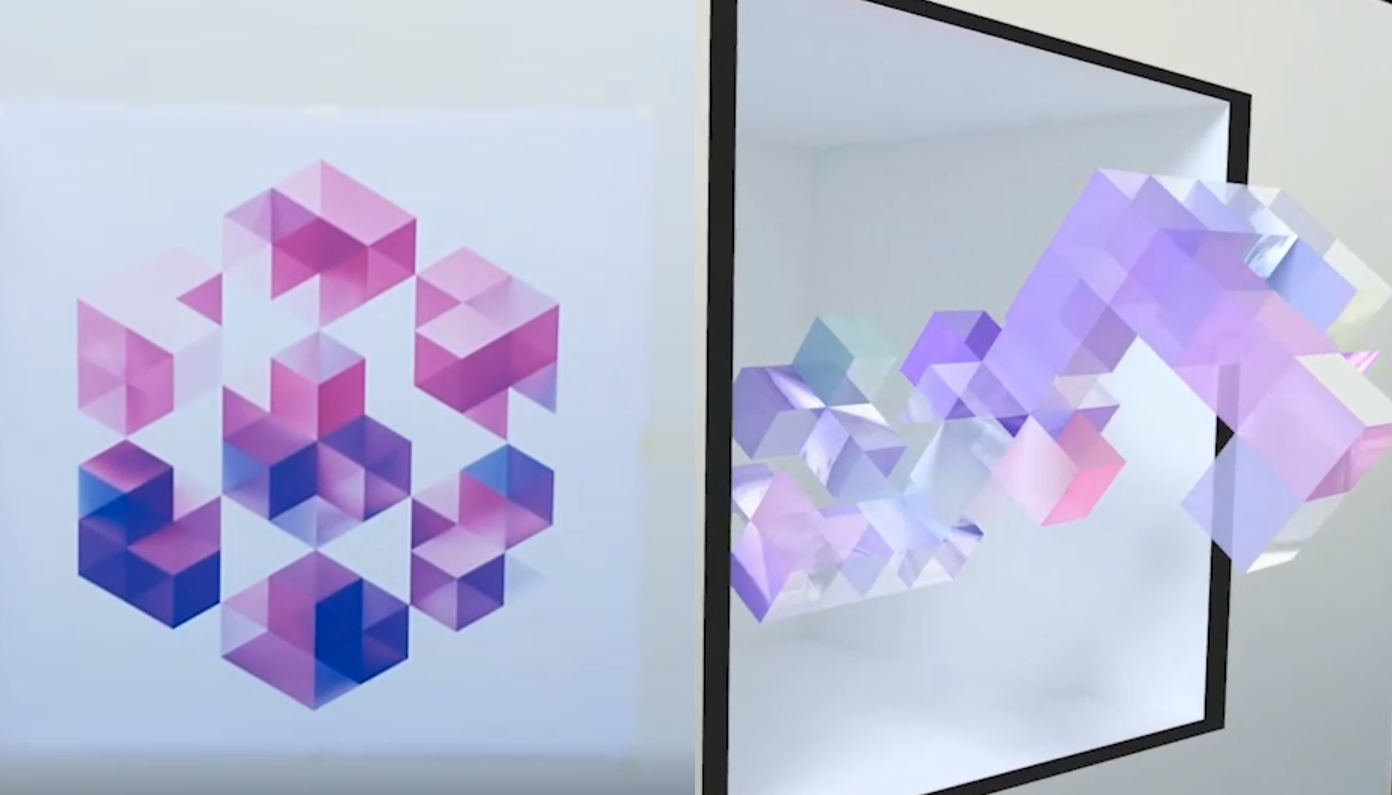
\includegraphics[scale=0.3]{augmented.png}
	\caption{Augmented Image mit ARCore, Bildquelle \cite{augmented_images}}
\end{figure} 

ARCore kann auch sich bewegende Bilder verfolgen, wie beispielsweise eine Plakatwand auf der Seite eines fahrenden Busses. Die Bilder können offline zusammengestellt werden, um eine Bilddatenbank zu erstellen, es ist jedoch auch möglich einzelne Bilder in Echtzeit vom Gerät hinzuzufügen. Nach der Registrierung erkannt ARCore diese Bilder, sowie die Grenzen dieser und gibt eine entsprechende Pose eines virtuellen Objekts zurück.

Mithilfe der \textbf{ARCore Cloud Anchor API} können kollaborative AR Multiplayer Anwendungen erstellt werden. Dazu wird von einem Gerät der Anker und die Features der näheren Umgebung in der Cloud gespeichert. Diese Anker können dann mit anderen Benutzern auf Android- oder iOS-Geräten in der selben Umgebung geteilt werden. Mit dieser Methode können zwei Endgeräte die gleiche virtuellen 3D Objekte an exakt der gleichen Stelle im Raum rendern, so dass beide Benutzer das gleiche Erlebnis teilen (vgl. \cite{fundamental_concepts}).

\subsection{Entwicklungsumgebungen}

ARCore kann mit vielen gängigen Entwicklungsumgebungen verwendet werden. Dazu zählen Android Studio, Android Native Development Kit, Unity für Android, Unity für iOS, Unreal Engine und iOS (vgl. \cite{develop}). Im Rahmen dieser Arbeit wurde Android Studio in der Version 3.4.1 verwendet.



\section{Sceneform}

\section{Google Location Service}

\section{Dexter}

\section{Volley}

\section{Implementierung}



